Dans cette première étape, nous chargeons une série de fichiers audio correspondant à différentes notes jouées par des instruments tels que le violon, la flûte et le piano. Ces fichiers audio sont ensuite convertis en signaux mono pour simplifier l'analyse. Pour chaque signal, nous calculons la puissance du signal en utilisant une fenêtre glissante de taille fixe. La puissance ainsi obtenue est ensuite convertie en décibels (dBm). Ce processus est essentiel pour préparer le signal en vue de l'analyse ultérieure. 
\begin{figure}[htb]
    \centering
    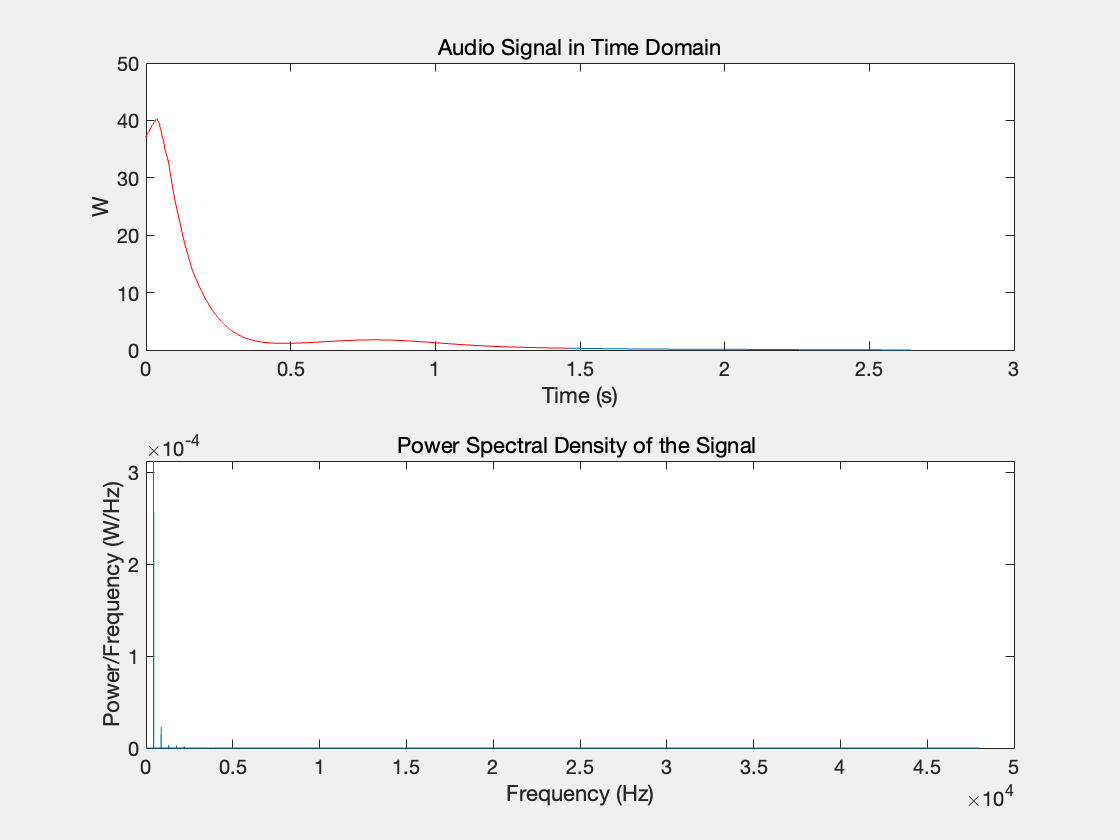
\includegraphics[width=0.8\textwidth]{Pi_A_96K.png}
    \caption{Spectre de puissance d'un signal audio(Piano)}
    \label{fig:Power_Spectrum}
\end{figure}